\documentclass[a4paper, 9pt, twoside, twocolumn]{article}

%%% PACKAGES %%%
\usepackage[utf8]{inputenc}
\usepackage[sc]{mathpazo}
\usepackage[T1]{fontenc}
\usepackage[english]{babel}
\usepackage[hmarginratio=1:1, top=32mm, columnsep=20pt, left=20mm, right=20mm]{geometry}
\usepackage[hang, small, labelfont=bf, up, textfont=it, up]{caption}
\usepackage{enumitem}
\usepackage{abstract}
\usepackage{titling}
\usepackage{hyperref}
\usepackage{graphicx}
\usepackage{epstopdf}

%%% PRE-DOCUMENT COMMANDS %%%
\setlist[itemize]{noitemsep}

\setlength{\droptitle}{-4\baselineskip}
\pretitle{\begin{center}\huge}
\posttitle{\end{center}}
\title{Learning Othello Board Evaluation with Artificial Neural Network}
\author{\textsc{Théo Verhelst}}

%%%% DOCUMENT CONTENT %%%
\begin{document}

\maketitle

\begin{abstract}
Othello (also named Reversi) is a board game that gained interest in research
for the simplicity of its rules and its interesting branching factor. Numerous
heuristics for board evaluation have been developed over the past decades, but
there is a growing trend towards the use of artificial neural networks (ANN) for
this purpose. We implemented minimax search algorithm with alpha-beta pruning
and simple heuristic in order to allow a human user to play Othello against a
competitive artificial player. We then used a multilayer neural network to learn
a board evaluation function, by using temporal difference learning (TDL) and
self-play. The ANN is used as the heuristic function of minimax search with a
ply depth of 1. Our ANN outperforms minimax search at ply depth of 6 with
carefully handcrafted heuristic.
\end{abstract}

\section{Introduction}
Our main focus was to study the use of artificial neural
network (ANN) as heuristic evaluation for minimax search. We chose to center the
search on the game Othello, since it has been well studied in the field of AI
and machine learning. Moreover, it has an interesting branching factor (around 7
on average \cite{Leouski1996}), which is not as big as in chess, but still big
enough to prevent us from doing exhaustive tree search. We came across the
article \cite{Binkly2007}, which is a great resource about state-of-the-art
Othello board evaluation with ANN. In this article, Binkly et al. claim that a
1-ply search is sufficient to compete against strong Othello players, if an
efficient neural network architecture is used. We decided to implement a basic
architecture, which, hopefully, will result in a decent Othello player.

An important part of the learning process in this kind of experiment is the way
data is extracted from game history, in order to be fed into the ANN. For this
purpose, Sutton et al. developed the Temporal Difference Learning (TDL)
\cite{Sutton1988}. TDL is used when predictions must be done in sequence, and
when the target value is available at the end of the sequence of predictions. We
use the current prediction to correct past ones, by supposing that more recent
prediction are more accurate, since we are closer in time to the outcome.

The rest of this document is outlined as follow. Section \ref{sec:othello} briefly
explains the rules of the Othello game. The TDL procedure is exposed more
precisely in section \ref{sec:tdl}. In section \ref{sec:nnet}, the details of
how ANNs are used for the purpose of board evaluation are investigated. The
setup of the experiment is given in section \ref{sec:experiment}, and its results
are given in section \ref{sec:results}.

\section{Othello game}
\label{sec:othello}
Othello is a two-players board game, played on a grid of 8 by 8 cells. The
player who plays first has black pieces, and the second player has white pieces.
The initial board is shown in figure \ref{othello_start}. Each turn, a player
puts one of its piece on an empty cell, in such a way as to capture at least one
of the opponent's pieces. A line of pieces is captured if it is bounded by
opponent's pieces at both ends. If no move leads to a capture, the game is over
and the player with the most pieces on the board wins.
\begin{figure}
    \centering
    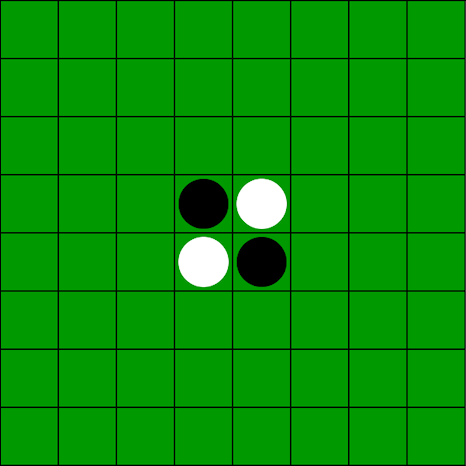
\includegraphics[width=0.75\linewidth]{othello}
    \caption{Initial board of the Othello game.\\
    Credits: \url{http://mnemstudio.org/game-reversi-intro.htm}}
    \label{othello_start}
\end{figure}

\section{Temporal Difference Learning}
\label{sec:tdl}
A major problem arises when one wants to use machine learning to play complex
board games such as Othello. A game is composed from a sequence of states, and
the role of the evaluation function is to learn whether a given game state is
likely to lead to a win. One could therefore train the model to predict a win
for all boards encountered in a game ending by a win, and similarly to predict a
loss for all boards encountered in a game ending by a loss. The main problem
with this approach is that there is a lot of uncertainty in games such as
Othello, and none of the players are perfect. Therefore, the correlation between a state in
the beginning of a game and the outcome of this game may be low \cite{Binkly2007}.

Temporal difference learning (TDL) \cite{Sutton1988} is a solution to this
issue. According to \cite{Binkly2007, Leouski1996}, the method TD($0$), which is a special
case of the TD($\lambda$) class of temporal difference methods, is the most
appropriate to learn from Othello games. Let $S$ be the set of all possible
board states,  $(s_1,s_2,\dots,s_n)\in S^n$ the sequence of states of a given
game, and $z$ the outcome of the game. Consider the sequence of states evaluated
by the first player. Since we are using 1-ply search, this sequence is $(s_2,
s_4, \dots)$. Let us rename this sequence $(v_1, v_2, \dots, v_m)$. The
evaluation of a state $v_t$ by the first player is denoted $f(w, v_t)$, where
$w$ is the weight vector of its evaluation function. The classical approach to
TD($0$) is to compute a weight increment at each turn using the formula given in
\cite{Sutton1988}:
\begin{equation}
    \Delta w_t=\alpha(f(w, v_{t+1}) - f(w, v_t))\nabla_w f(w, v_t)\quad\forall t\in\{1,\dots,m\}
\end{equation}
where $f(w, v_{m+1}) := z$, and $\alpha$ is the learning rate. We have then to
update $w$ at the end of the game, when the outcome $z$ is known
\begin{equation}
    w\leftarrow w+\sum_{t=1}^m \Delta w_t
\end{equation}

However, this approach was difficult to apply to our study. Indeed, we used a
neural network library for Java called Neuroph, and it does not include temporal
difference learning out of the box. A lot more effort would therefore have been
needed to implement this learning rule. Instead, we used the approach explained
in \cite{Steeg2015}, which consist of learning to predict the evaluation of
current board $f(w, v_t)$ when the previous board state $v_{t-1}$ is given as
input. The pairs $(v_{t-1}, f(w, v_t))$ are stored while the game is running,
and the model learns from them once the game is finished. This approach and the
one given in \cite{Sutton1988} are equivalent, and the difference is in fact
an implementation detail.

\section{Neural Network for Board Evaluation}
\label{sec:nnet}
Numerous ANN architectures have been studied for the purpose of learning Othello
board evaluation \cite{Binkly2007, Leouski1996}. The one we chose is the first
one described in \cite{Leouski1996}. We selected this architecture for its
simplicity. It consists solely of 64 inputs units, one for each of the board
cells, one hidden layer of 50 units, and one output unit. The board is encoded
by a number for each board cell, where $0$ accounts for an empty cell, $1$ for
a cell with the player's piece, and $-1$ for a cell with the opponent's piece.
The game outcome $z$ is encoded similarly: $1$ for a win, $-1$ for a loss and $0$
for a draw.

According to the results of \cite{Binkly2007}, a network input consisting of 2
or 3 input units per board cell outperforms the approach described above, given
equivalent ANN architectures. Therefore, we used the following board encoding
described in \cite{Binkly2007}: $(1, -1)$ for the player's pieces, $(-1, 1)$ for
the opponent's pieces and $(-1, -1)$ for an empty cell.

There is some other features that we could have used in order to improve our
ANN, most of them are described in \cite{Binkly2007}: weight sharing to account
for board symmetry, symmetry removal, spatial processing layer, multiple hidden
layers, exhaustive minimax search at the end of the game. However, we chose not
to implement any of them for time constraint reasons.

We used a naive solution to account for board symmetry, which has not been
proposed in any of the referenced articles. When a board is proposed to the ANN
for learning, all of the 8 symmetries of this board \cite{Binkly2007} are
generated, and they are also proposed for learning to the ANN with the same
target value. This method resulted in a slight performance increase.

\section{Experimental Setup}
\label{sec:experiment}
We followed the training methodology given in \cite{Binkly2007}, which consists
of making two ANNs playing against each other, learning from the games according
to the TD($0$) method, and frequently evaluating their performance against a
reference player. The reference player we used is described in \cite{Binkly2007}
and \cite{Yoshika1999}. \footnote{Blinkly et al. claim in \cite{Binkly2007} that
this reference player originated from \cite{Yoshika1999}. However, the table in
figure \ref{heuristic_board} is not to be found in \cite{Yoshika1999}, while the
equation \ref{ref_player} is indeed present. Therefore, we give the credit of
this reference player to both articles.}. It uses minimax search at ply depth of 3 with a
handcrafted heuristic function, which is defined for some board state $x$ by
\begin{equation}
\label{ref_player}
f(x) = \sum_{i=1}^{64} w_i x_i + N(0, \sigma_{noise})
\end{equation}
where $N(0, \sigma_{noise})$ is Gaussian noise with mean $0$ and standard
deviation $\sigma_{noise}$, and $w_i$ is defined according to the table in
figure \ref{heuristic_board}.

\begin{figure}
    \centering
    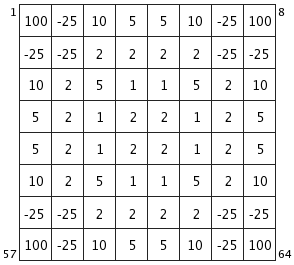
\includegraphics[width=0.75\linewidth]{heuristic_board}
    \caption{Weights of the heuristic function used by the reference player. Credits:
        \cite{Binkly2007}.}
    \label{heuristic_board}
\end{figure}

We trained two ANNs against each other in 45,000 successive games, and one of them
played 50 games against the reference player every 150 training games, in order
to evaluate the evolution of the ANNs performance.

In the learning process, $\epsilon$-decreasing move choice policy
\cite{Scott2010} has been used. In the first game, the ANNs choose the estimated
optimal move with probability $1-\epsilon=0.9$, and selects a random one with
probability $\epsilon=0.1$. As the learning process runs, the value of
$\epsilon$ decreases linearly, and finally reaches $0$ in the last game of the
training process.

\section{Results and Discussion}
\label{sec:results}
\begin{figure*}
    \centering
    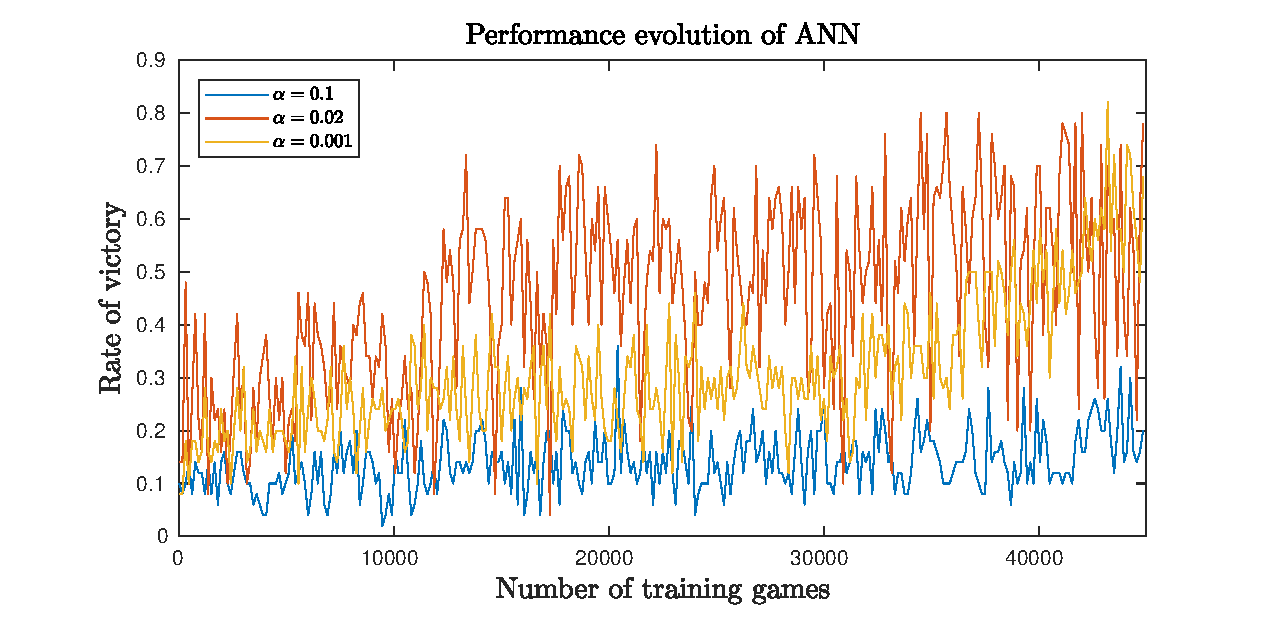
\includegraphics[width=\linewidth]{final_not_smoothed}
    \caption{Evolution of the winning rate against the reference player, for
    various values of the learning rate.}
    \label{non_filtered}
\end{figure*}
\begin{figure*}
    \centering
    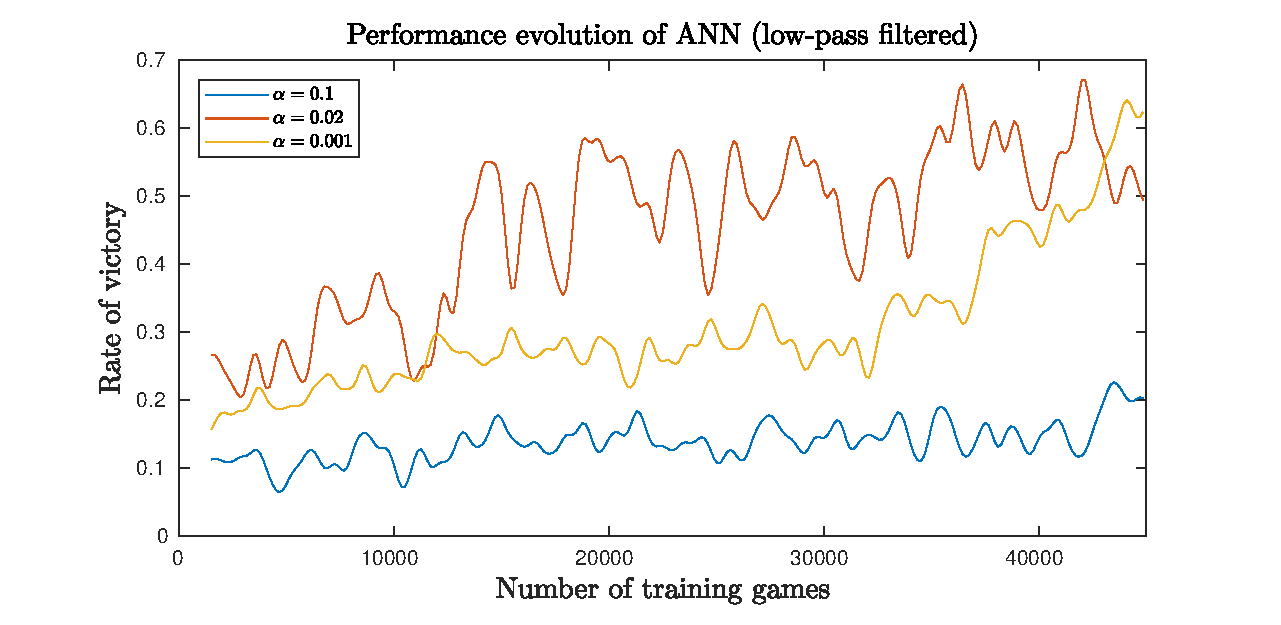
\includegraphics[width=\linewidth]{final_smoothed}
    \caption{Evolution of the winning rate against the reference player, for various
    values of the learning rate. The data
    has been filtered with a Gaussian filter with window of width 825.}
    \label{filtered}
\end{figure*}

Results of the experiment are shown in figure \ref{non_filtered} and
\ref{filtered}. The winning rate evolution in figure \ref{non_filtered} is very
noisy, we thus filtered the sequence with a low-pass filter in figure
\ref{filtered}, in order to see more clearly the progression. We first ran the
whole learning process with a learning rate $\alpha=0.1$. We noticed that the
the performance was not stable and did not evolve noticeably. Therefore, we
found two other promising values by grid search, $\alpha=0.02$ and
$\alpha=0.001$. While $\alpha=0.02$ leads to quicker learning than
$\alpha=0.001$, its also results in less stable performance. When comparing the
three curves, it is clear that $\alpha=0.1$ results in an overshooting of the
optimal weights, and therefore the convergence was not attained.

It seems that our ANN player finally outperformed the minimax player by reaching
a winning rate greater than 0.5. That indicates that the neural network learned
from the raw board input features at least as efficient as a carefully
handcrafted heuristic developed by experts.

Another important aspect of these results is that we were not able to formally
assess the influence of various features we implemented, such as the number of
input per board cell, the number of hidden neurons, the training procedure, and
so forth. We relied on the results of previous studies when it came to decide
whether or not to use them. Ideally, we would had run the same training process
with and without them, in order to make sure that they are relevant to our
problem.

\begin{table}
    \centering
    \begin{tabular}{lll}
        Ply depth & ANN 1 & ANN 2\\
        \hline
        1 & 0.65 & 0.53 \\
        2 & 0.58 & 0.65 \\
        3 & 0.65 & 0.7 \\
        4 & 0.69 & 0.56 \\
        5 & 0.81 & 0.71 \\
        6 & 0.76 & 0.7 \\
        \hline
    \end{tabular}
    \caption{Winning rate of both trained ANN with $\alpha=0.02$ against the reference player with
            various ply depths.}
    \label{tab02}
\end{table}

Once the ANNs has been trained, we ran test games between both neural network
players and the reference player at various ply depth. Each winning rate has
been calculated from 100 test games. Surprisingly, the ply depth of the opponent
does not seem to influence the winning rate of the ANN player. This may be
explained by the fact that we use TDL methods, which may be thought as having an effect
approximating a minimax search with infinite ply depth. Indeed, by indirectly
back-propagating the final outcome of a game to all boards in the history of the
game, the neural network learns which kind of board usually leads to a win, and
conversely. This approximation becomes better as the game comes closer to
its end.

\newpage
\footnotesize
\bibliographystyle{ieeetr}
\bibliography{doc}

\end{document}
